\documentclass[10pt,a4paper]{report}
\usepackage[latin1]{inputenc}
\usepackage{amsmath}
\usepackage{amsfonts}
\usepackage{amssymb}
\usepackage{graphicx}
\usepackage{enumitem}
\newlength{\figwidth}
\setlength{\figwidth}{0.9\columnwidth}

\newlength{\qfigheight}
\setlength{\qfigheight}{0.25\textheight}

\newlength{\hfigheight}
\setlength{\hfigheight}{0.5\textheight}
\author{}
\title{Analyzer feedback to track-efficiency systematic}
\date{}
\begin{document}
	\maketitle
\begin{itemize}
	\item[1.] \underline{The procedure}: The procedure of changing binning and/or cut parameters to evaluate systematic uncertainties is common practice and should not need explanation. The specific method of calculating an uncertainty from 2 experimentally unknown values is also common practice. If the committee is referring to the procedure of the track-efficiency calculation itself, then please clarify. However, if its a list of plots on the procedure that is desire, then I implore the committee to explain which plots are desired. The only ones available are the 
	\begin{itemize}
		\item Efficiency of the data reconstruction for $p$;$\pi^{+}$;$\pi^{-}$
		\item Efficiency of the Monte-Carlo reconstruction for $p$;$\pi^{+}$;$\pi^{-}$
		\item Ratio of Efficiencies of the Monte-Carlo reconstruction for $p$;$\pi^{+}$;$\pi^{-}$
	\end{itemize}
	However if the committee just wished for a "data dump" of these plots, then one will be provided.
	\item[2.] \underline{The estimate}: Clarify please as there is no "well formulated problem" i.e. text-book like occurrence in the manuscript.
	\begin{itemize}
		\item[a.] Correct, this is stated in the note Sec. 6.1.
		\item[b.] Correct, hence why analyzer chose a four-dimensional binning scheme.
		\item[c.] Correct that is is not statistical. However incorrect about "\textbf{Nonetheless, you are going to use a random method to estimate it}". This is not a random method. Analyszer implores comitte to read or skim through "Data Analysis in High Energy Physics: A practical Guide to Statistical Methods" ISBN:978-3-527-41058-3. Also, I do not let the cause of the uncertainty randomly vary and also from the context of this bullet point, it is clear that the procedure of calculating this systematic is lost on the committee, Therefore I request a meeting.
		\item[d.] Invalid because c is misinterpreted.
	\end{itemize}
	\item[3.] \underline{The method}:
		\item[a.] Almost correct. There is no "nominal" choice or the correction, hence why the percent error method was chosen. By stating a "nominal value" you are stating that one value is known, which in this case it is not known which correction is correct. All we know is that either correction can be the correct one.  Also, the bin width is varied with between the two sets of corrections.
		\item[b.] The "ideal method" described is a matter of preference and is not "ideal" to the analyzer. The rest of this bullet is correct.
	\item[4.] \underline{The interpretation }:
			\item[a.] The cause of the non-Gaussian shape is a simple concept as the track-efficiency populates $p$;$\pi^{+}$;$\pi^{-}$ phasespace and the events that needed a track-efficiency correction were populated by the channel $p \pi^{0} \to p e^{+}e^{-}(\gamma)$, which is governed by the $\pi^{0}$ cross-section. But lets stay focused on the committees "ideal".  
			\item[b.] Refused: As seen on the plot given above, the mean, as calculated by ROOT, which is as committee wants, is lower in value than the analyzer wants to report. Also this value does not statistically capture the true value of the correction.
			\item[c.] This comment by the committee is also incorrect. Also refused to use the RMS in quadrature because the RMS, is the error of the error. 
			 \begin{figure}[h!]\begin{center}
					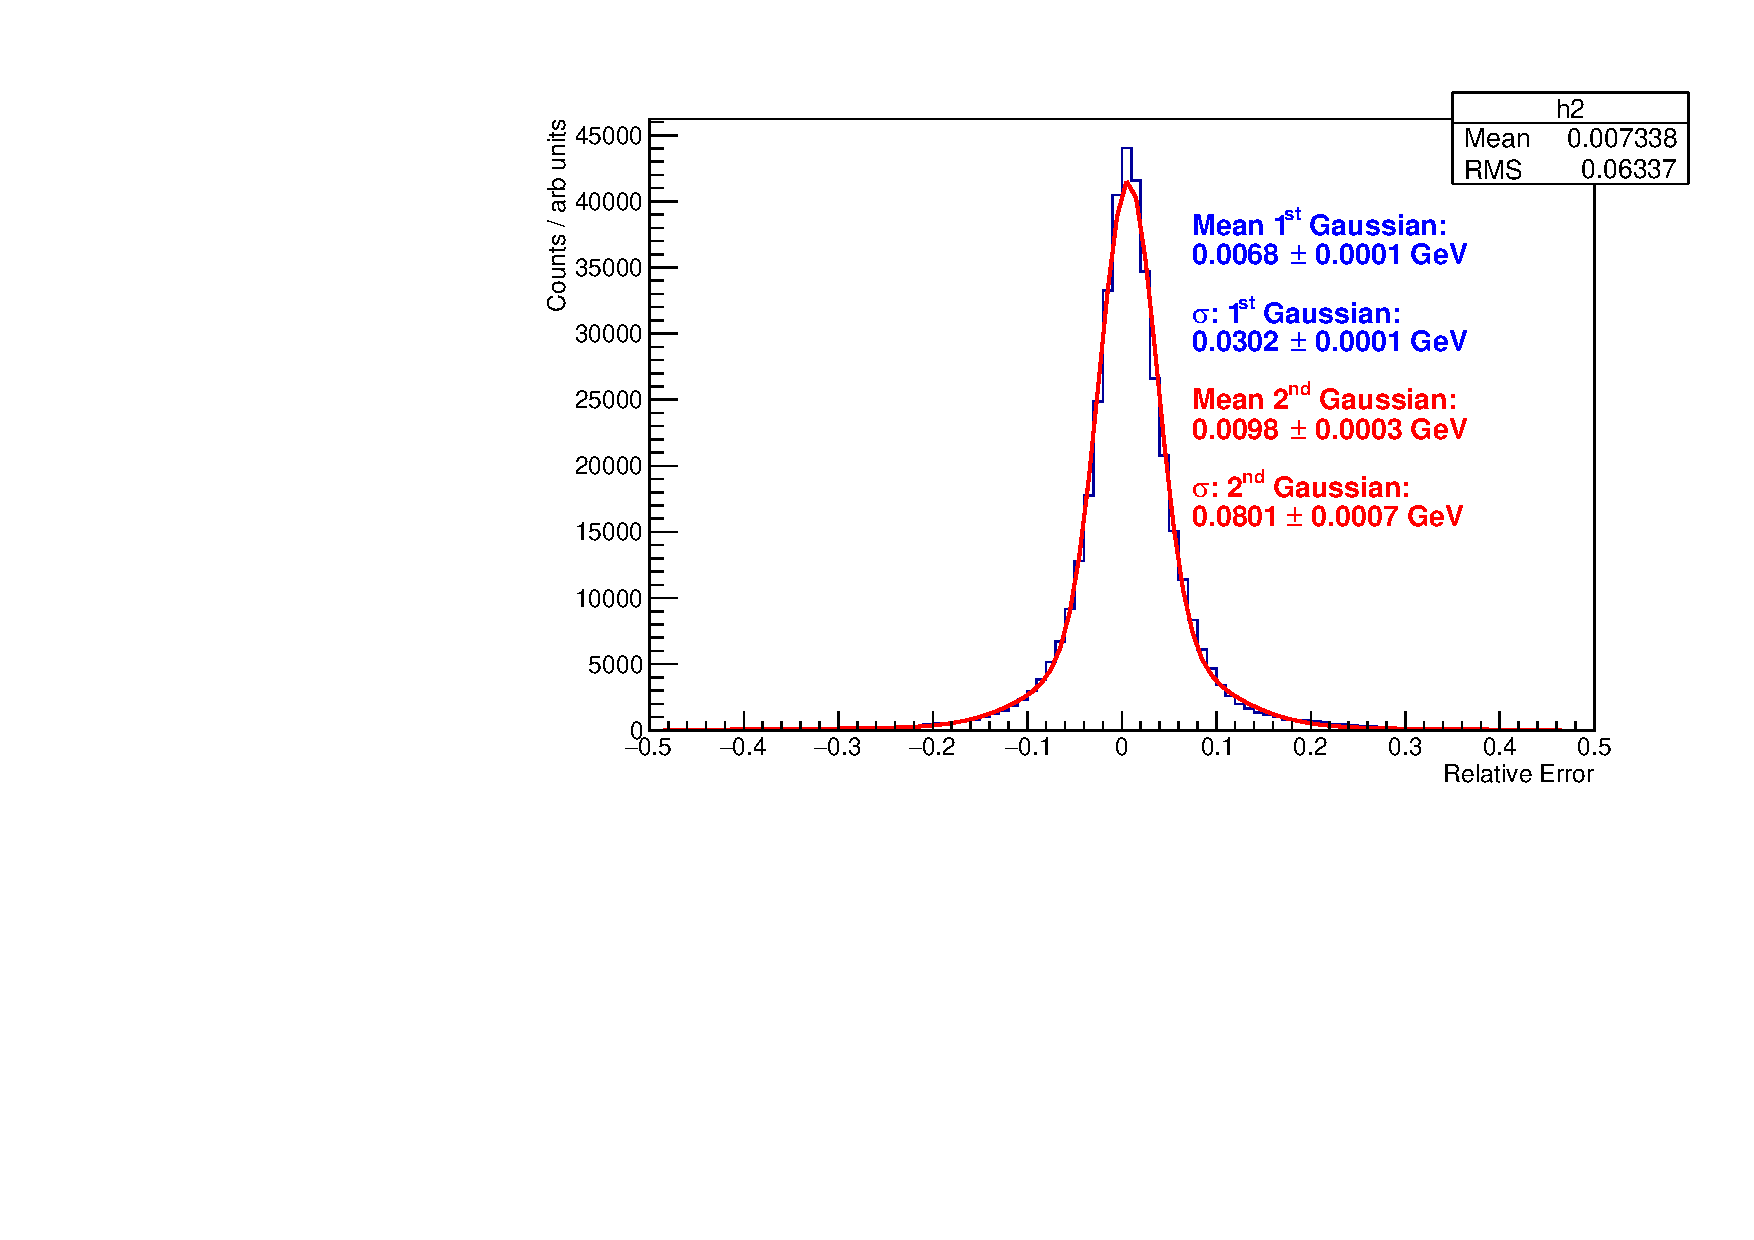
\includegraphics[width=1.1 \figwidth,height=\hfigheight]{/Users/michaelkunkel/WORK/GIT_HUB/Pi0_Papers/ANALYSIS_NOTE/RESULTS/NewEffPlotSyswstats.pdf}
					\caption{Relative error calculated between the two sets of track efficiencies.}\label{fig:toteff_error}
				\end{center}\end{figure}
	\item[5.] \underline{Communication}: Analyzer confused by this statement. Requests meeting.
\end{itemize}
\end{document}